\documentclass{article}
\usepackage{arxiv}

\usepackage[utf8]{inputenc}
\usepackage[english]{babel}
\usepackage[T1]{fontenc}
\usepackage{url}
\usepackage{booktabs}
\usepackage{amsfonts}
\usepackage{nicefrac}
\usepackage{microtype}
\usepackage{lipsum}
\usepackage{graphicx}
\usepackage{natbib}
\usepackage{doi}
\usepackage{amsmath}
\usepackage{amsthm}
\usepackage{algorithm}
\usepackage{algpseudocode}

\newtheorem*{assumption*}{\assumptionnumber}
\providecommand{\assumptionnumber}{}
\makeatletter
\newenvironment{assumption}[2]
 {%
  \renewcommand{\assumptionnumber}{\textbf{Assumption} #1 ({#2})}%
  \begin{assumption*}%
  \protected@edef\@currentlabel{#1-#2}%
 }
 {%
  \end{assumption*}
 }


\title{A template for the \emph{arxiv} style}

\author{ Kreinin M. \\
	Department of Intelligent Systems\\
	MIPT\\
	Moscow, Russia \\
	\texttt{kreinin.mv@phystech.edu} \\
}
\date{}

\renewcommand{\shorttitle}{\textit{arXiv} Template}

%%% Add PDF metadata to help others organize their library
%%% Once the PDF is generated, you can check the metadata with
%%% $ pdfinfo template.pdf
\hypersetup{
pdftitle={A template for the arxiv style},
pdfsubject={q-bio.NC, q-bio.QM},
pdfauthor={Kreinin M.},
pdfkeywords={First keyword, Second keyword, More},
}

\begin{document}
\maketitle

\begin{abstract}
	This paper examines the convergence rate of adaptive gradient methods when a regularization function is added to the target function. This is an area of research, since many machine learning problems use the heuristic, heuristic regularization, and we investigate the theoretical and practical convergence of adaptive gradient methods.
\end{abstract}

\keywords{Adam \and OASIS \and Regularization \and ADAHessian}

\section{Introduction}
In machine learning we consider optimization problem
\begin{equation*}
	\min_{w \in \mathbb{R}^d} f(w)
\end{equation*}
Problems of the form (1) cover a plethora of applications, including empirical risk minimization,
deep learning, and supervised learning tasks such as regularized least squares or logistic regression. This minimization problem can be difficult to solve, particularly when the number of training
samples n, or problem dimension d, is large, or if the problem is nonconvex.

There are second order preconditioners methods for solving this problem, such as Adam, OASIS, AdaHessian. 

Throughout this work we assume that each f $:\mathbb{R}^d \rightarrow \mathbb{R}$ is twice differentiable and also L-smooth. This is formalized in the following assumption.

\begin{assumption}{1}{Convex}
	The function f is convex, i.e. $\forall w, w' \in \mathbb{R}^d$
	\begin{equation}
		f(w) \geq f(w') + \langle \nabla F(w'), w-w' \rangle
	\end{equation}
\end{assumption}

\begin{assumption}{2}{L-smoothness}
	The gradients of F are L-Lipschitz continuous $\forall w \in \mathbb{R}^d$, i.e. there exists a constant $L > 0$ such that $\forall w, w' \in \mathbb{R}^d$,
	\begin{equation*}
		f(w) \leq f(w') + \langle \nabla f(w'), w-w' \rangle + \frac{L}{2} ||w - w'||^2
	\end{equation*}
\end{assumption}

\begin{assumption}{3}{Twice differentiable}
	The function f is twice continuously differentiable.
\end{assumption}

\begin{assumption}{4}{$\mu$ - strongly convex}
	The function f is $\mu$-strongly convex, i.e., there exists a constant $\mu > 0$ such that $\forall w, w' \in \mathbb{R}^d$
	\begin{equation*}
		f(w) \geq f(w') + \langle f(w'), w-w' \rangle +\frac{\mu}{2} ||w - w'||^2
	\end{equation*}
	
\end{assumption}


\section{Problem statement}
We consider the unconstrained optimization problem
\begin{equation*}
	\min_{w \in \mathbb{R}^d} f(w)
\end{equation*}
Problems of the form cover a plethora of applications, including empirical risk minimization,
deep learning, and supervised learning tasks such as regularized least squares or logistic regression.

But we can add regulirazation $r(w)$ -- regularization, and solve the unconstrained optimization problem.
\begin{equation*}
	\min_{w \in \mathbb{R}^d} F(w) = f(w) + r(w)
\end{equation*}

For solving these problems we always scaled adaptive gradients algorithms like ADAM, OASIS, ADAHessian. We investigate how the convergence rate will change when the regularization function is added to these algorithms.
\if 0
\begin{algorithm}[H]
	\caption{Based algorithm}\label{alg:Based}
	$w_0, D_0, \eta_0$
	\begin{algorithmic}
		\For{$k = 1, 2, ...$}
		\State $D_k$ - update
		\State $\eta_k$ - update
		\State Set $w_{k+1} = w_k - \eta_k D_k^{-1} \nabla F(w_k)$
		\EndFor
	\end{algorithmic}
\end{algorithm}
\fi

\if 0
Examples of similars algorithms.
\begin{algorithm}[H]
	\caption{Adam}\label{alg:Adam}
		\begin{algorithmic}
		\Require{$\alpha, \beta_1, \beta_2, \epsilon, f$}
		\State $m_0 = 0$ -- 1-st moment vector
		\State $v_0 = 0$ -- 2-nd moment vector
		\State $t = 0$ -- timestep
		
		\While {$\theta$ not converged}
			\State $t = t+1$
			\State $g_t = \nabla_{\theta} f_t(\theta_{t-1})$
			\State $m_t = \beta_1 \cdot m_{t-1} + (1 - \beta_1) \cdot g_t$
			\State $v_t = \beta_2 \cdot v_{t-1} + (1 - \beta_2) \cdot g_t^2$
			\State $\hat{m_t} = \frac{m_t}{1-\beta_1^t}$
			\State $\hat{v_t} = \frac{v_t}{1-\beta_2^t}$
			\State $\theta_t = \theta_{t-1} - \alpha \cdot \frac{\hat{m_t}}{\sqrt{v_t} + \epsilon}$
		\EndWhile
	\end{algorithmic}
	\end{algorithm}
	
	\begin{algorithm}[H]
	\caption{OASIS}\label{alg:OASIS}
	\begin{algorithmic}
		\Require{$w_0, \eta_0, D_0, \theta_0 = + \infty$}    
		\State $w_1 = w_0 - \eta \hat{D_0}^{-1} \nabla F(w_0)$
	
		\For{$k = 1, 2, ...$}
		\State $D_k = \beta D_{k-1} + (1-\beta_2) \cdot diag\left( z_k \odot \nabla^2 F(w_k) z_k \right)$
		\State $(\hat{D_k})_{ii} = max \{|D_k|_{i, i} ; \alpha \}$, $\forall i = \overline{1, d}$
		\State $\eta_k = min \{ \sqrt{1 + \theta_{k-1}} \cdot \eta_{k-1}; \frac{||w_k - w_{k-1}||_{\hat{D_k}}}{2 ||\nabla F(w_k) - \nabla F(w_{k-1}) ||_{\hat{D_k}}^* } \}$
		\State $\theta_k = \frac{\eta_k}{\eta_{k-1}}$
		\EndFor
		
	\end{algorithmic}
\end{algorithm}
\fi

% В исследуемом нами алгоритме сходимости мы будем исследовать алгоритмы двух следующих видов. В первом функция регуляризации выносится отдельном в пересчете весов модели, во втором функция домножается на обратный "гессиан".
In the convergence algorithm that we study, we will investigate algorithms of the following two kinds. In the first one, the regularization function is taken out separately in the recalculation of model weights, and in the second one, the function is dominated by the inverse "hessian".

\begin{algorithm}[H]
	\caption{Based algorithm}\label{alg:Based}
	$w_0, D_0, \eta_0$
	\begin{algorithmic}
		\For{$k = 1, 2, ...$}
		\State $D_k$ - update by using information of $f(w)$
		\State $\eta_k$ - update
		\State Set $w_{k+1} = w_k - \eta_k D_k^{-1} \nabla f(w_k) - \eta \nabla r(w)$ 
		\State or like that
		\State Set $w_{k+1} = w_k - \eta_k D_k^{-1} (\nabla f(w_k) + \nabla r(w))$
		\EndFor
	\end{algorithmic}
\end{algorithm}



%\section{Headings: first level}
%\label{sec:headings}
% See Section \ref{sec:headings}.
%\subsection{Headings: second level}
%\subsubsection{Headings: third level}
%\paragraph{Paragraph}
%\section{Examples of citations, figures, tables, references}
%\label{sec:others}

\subsection{Citations}

\cite{kingma2014adam}, \cite{jahani2021doubly}, \cite{sadiev2022stochastic}, \cite{beznosikov2022scaled}, \cite{stich2019unified}

%\subsection{Figures}
%See Figure \ref{fig:fig1}. Here is how you add footnotes. \footnote{Sample of the first footnote.}
%\begin{figure}
	%\centering
	%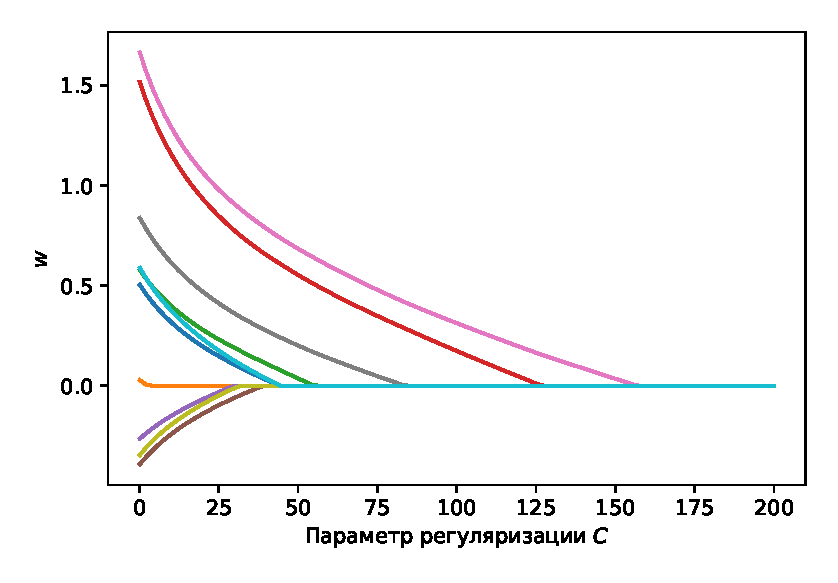
\includegraphics[width=0.5\textwidth]{../figures/log_reg_cs_exp.eps}
	%\caption{Sample figure caption.}
	%\label{fig:fig1}
%\end{figure}

%\subsection{Tables}
%See awesome Table~\ref{tab:table}.
%The documentation for \verb+booktabs+ (`Publication quality tables in LaTeX') is available from:
%\begin{center}
%	%\url{https://www.ctan.org/pkg/booktabs}
%\end{center}

\if 0
\begin{table}
	\caption{Sample table title}
	\centering
	\begin{tabular}{lll}
		\toprule
		\multicolumn{2}{c}{Part}                   \\
		\cmidrule(r){1-2}
		Name     & Description     & Size ($\mu$m) \\
		\midrule
		Dendrite & Input terminal  & $\sim$100     \\
		Axon     & Output terminal & $\sim$10      \\
		Soma     & Cell body       & up to $10^6$  \\
		\bottomrule
	\end{tabular}
	\label{tab:table}
\end{table}
\fi
\if 0
\subsection{Lists}
\begin{itemize}
	\item Lorem ipsum dolor sit amet
	\item consectetur adipiscing elit.
	\item Aliquam dignissim blandit est, in dictum tortor gravida eget. In ac rutrum magna.
\end{itemize}
\fi

\bibliographystyle{unsrtnat}
\bibliography{references}

\end{document}